% !TeX root = repressed-anger.tex

\section{Sentiment Analysis}
\label{sec:sentiment_analysis}

\acrfull{sa}, sometimes referred as \acrfull{om}, is the field of study that aims determine the attitude of the author respect to some topic. During the last decade, due mainly to the rapid increase of the social media, the research of this area, which includes linguistics and \acrfull{nlp}, has gain more relevance as it has a wide range of applications that can be used commercially.

Almost the human actions are influenced by opinions. A practical example of this behavior that get repeated in daily basics occurs when before making a decision we want to know other' to contrast our thoughts. In business, when an organization requires to public or consumer opinion, it conducted different types of surveys to gather this information. However, nowadays we do not precise to ask personally to people around us to discuss about a product. Thanks to micro-blogs, Twitter and reviews in social networks, we can broaden the amount of external opinions for decision making. Due to the amusing amount of information available, sometimes we could face some challenges, such as finding reliable sources summarizing and filtering the relevant information. The same way we consume this information, companies also search for new ways to obtain and process such information efficiently without human intervention, to achieve this automated analysis is needed\cite{liu2012sentiment}.

\begin{figure}[!htp]
  \center
  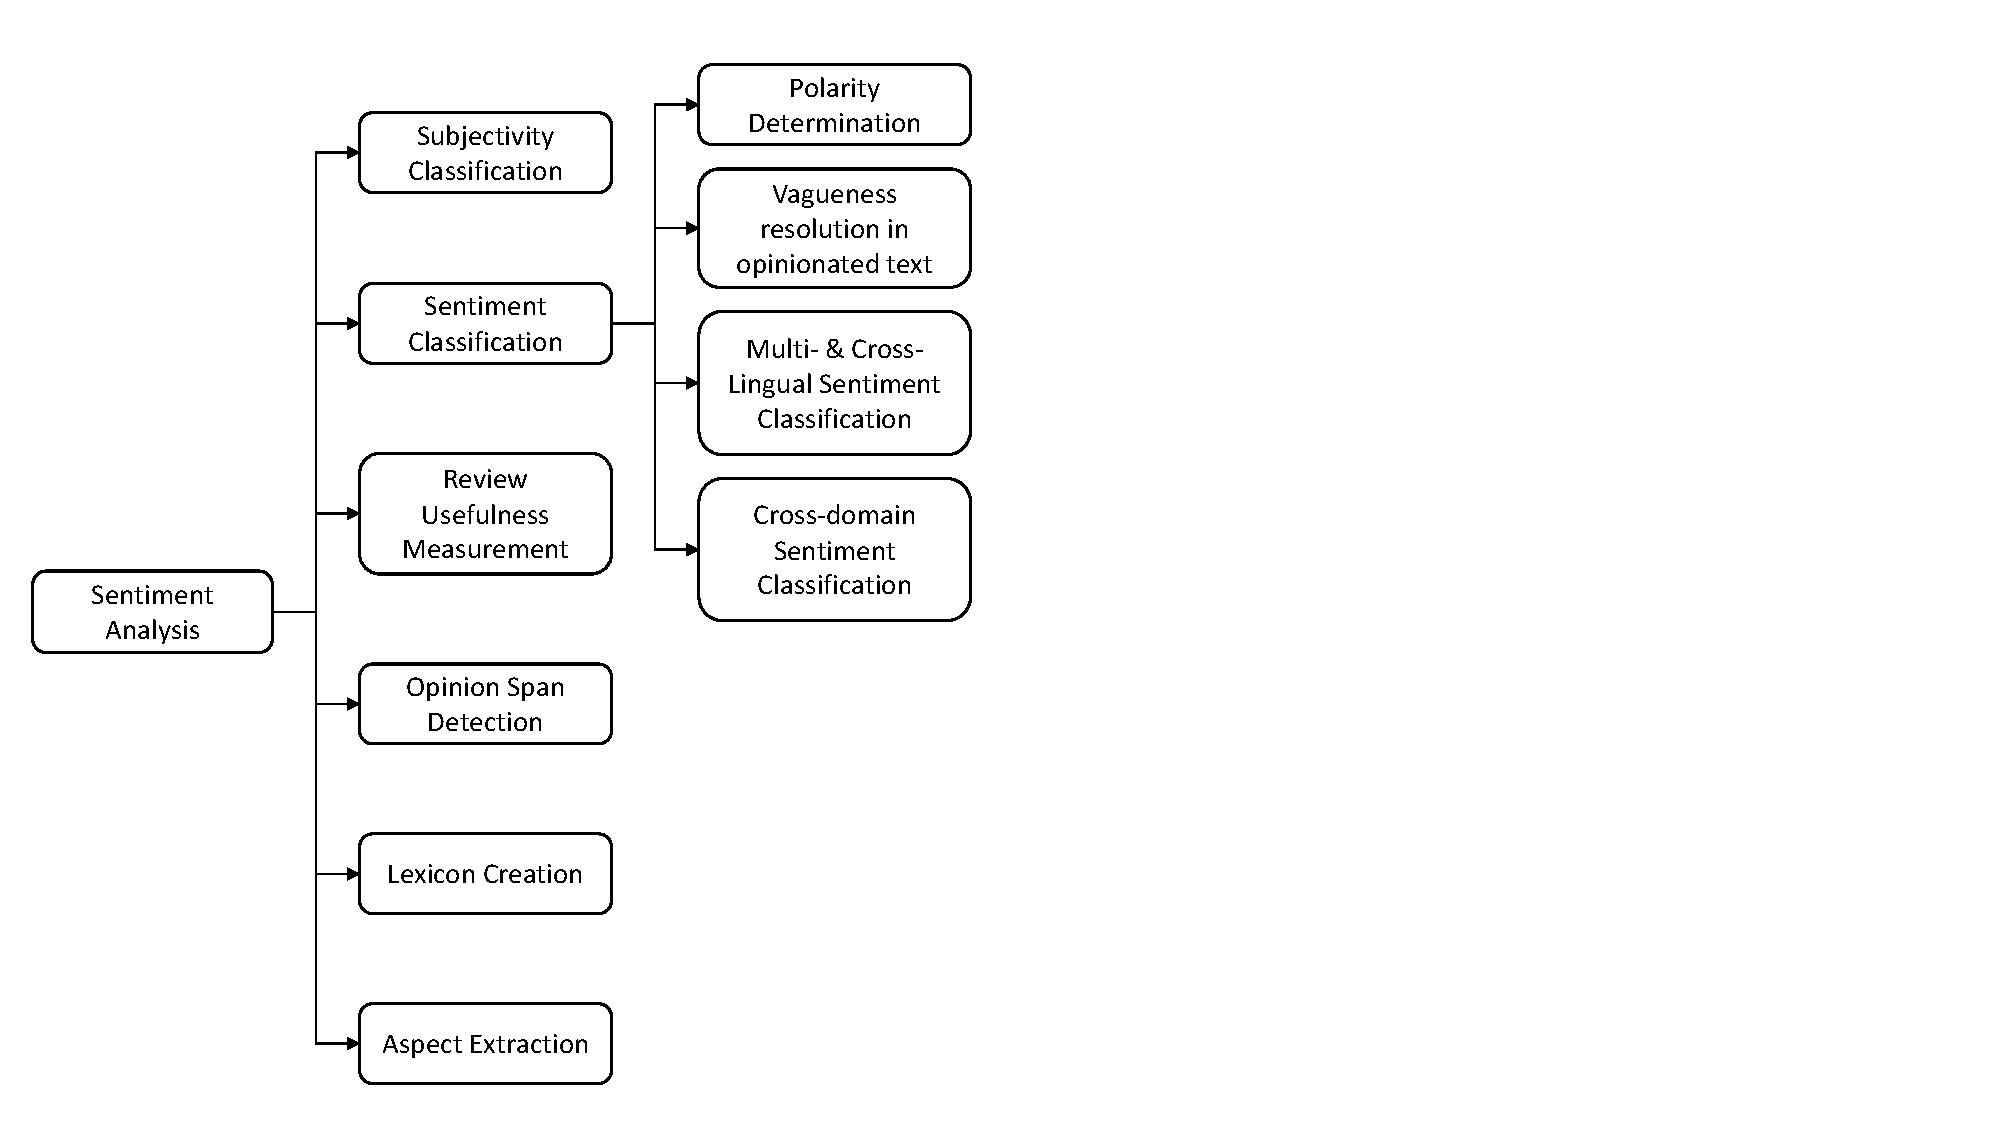
\includegraphics[width=0.6\textwidth]{figures/sentiment_analysis_tasks}
  \caption{Sentiment analysis tasks\cite{ravi2015survey}.}
  \label{fig:sentiment_analysis_tasks}
\end{figure}

\begin{figure}[!htp]
  \center
  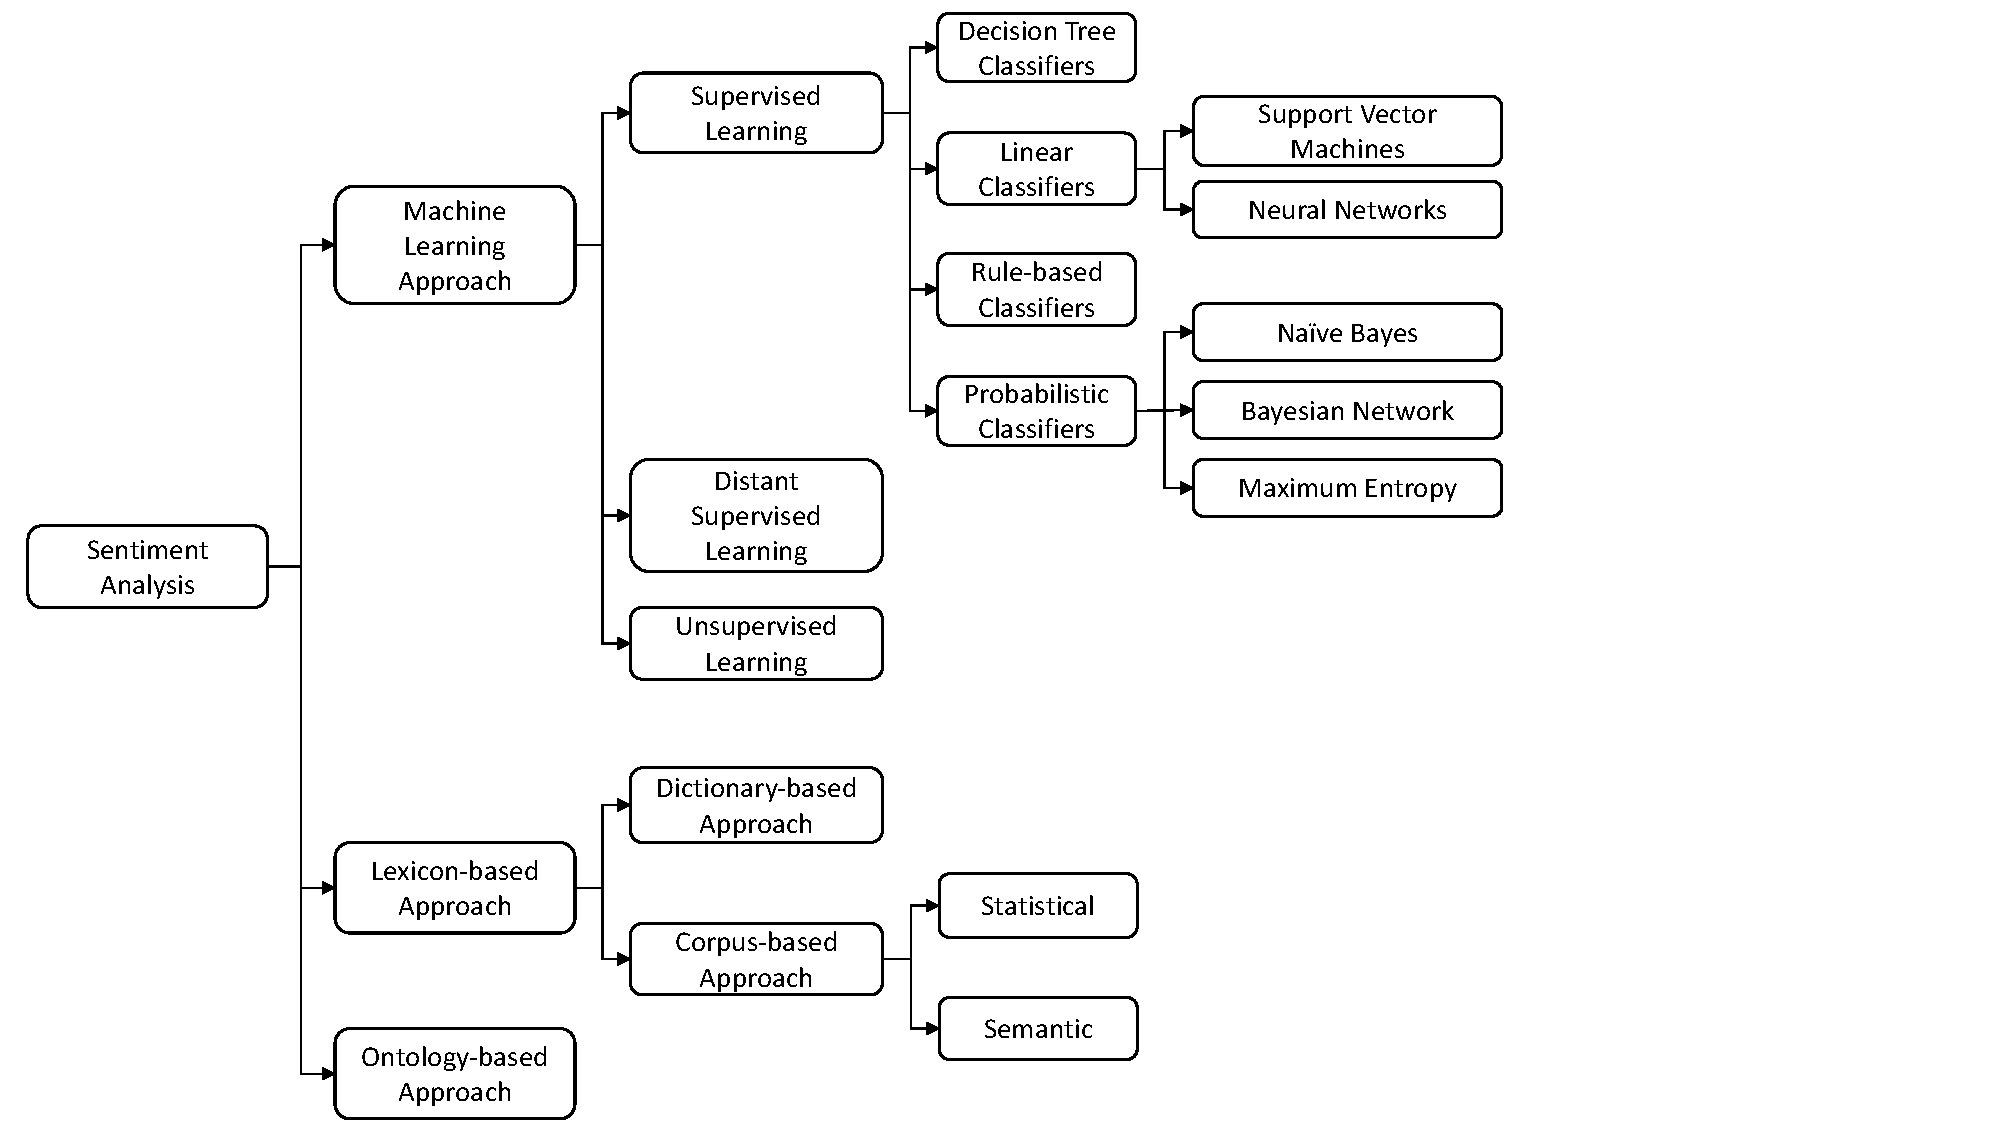
\includegraphics[width=1\textwidth]{figures/sentiment_analysis_techniques}
  \caption{Sentiment analysis techniques\cite{medhat2014sentiment}.}
  \label{fig:sentiment_analysis_techniques}
\end{figure}

\begin{figure}[!htp]
  \center
  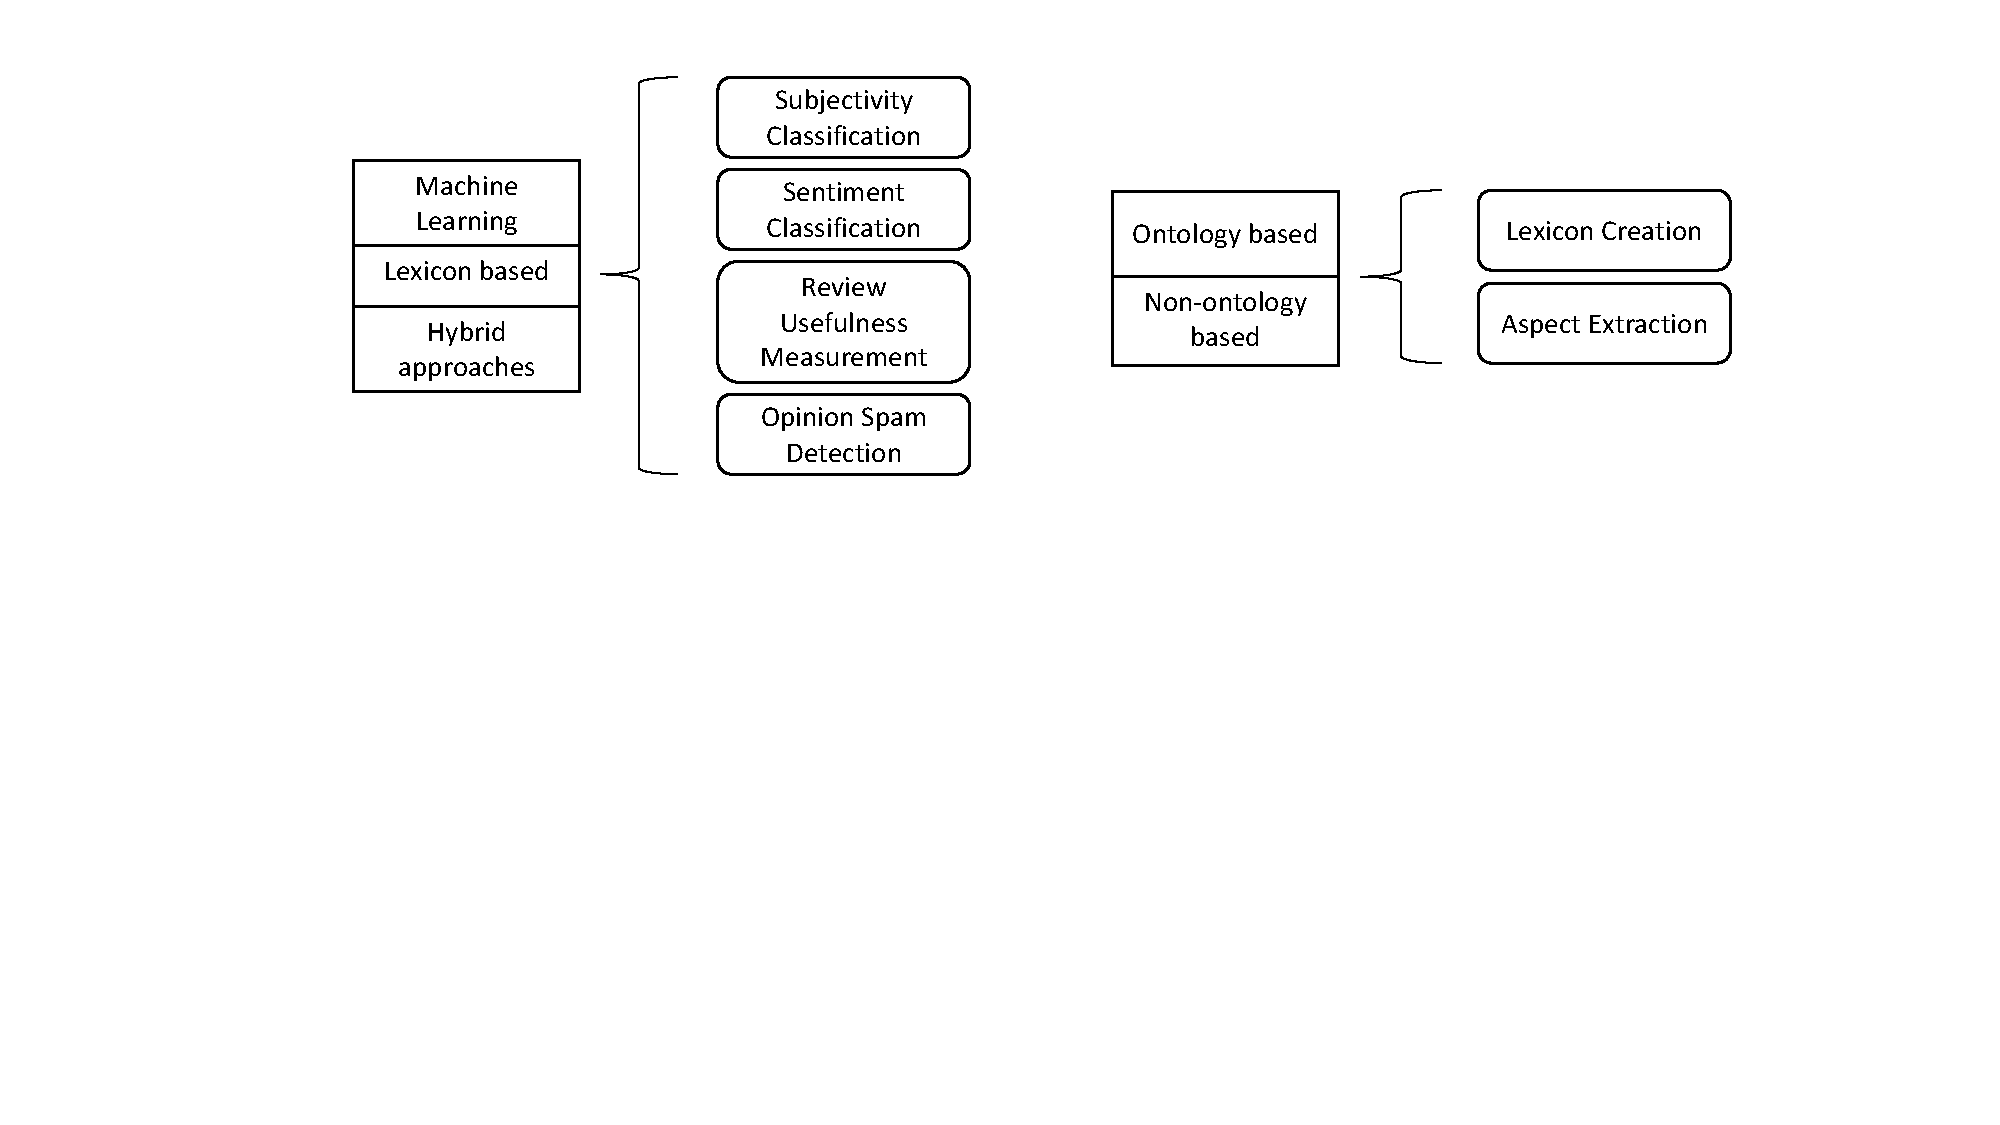
\includegraphics[width=0.4\textwidth]{figures/sentiment_analysis_approaches}
  \caption{Sentiment analysis approaches for each task.}
  \label{fig:sentiment_analysis_approaches}
\end{figure}

\cite{tripathy2016classification}
\cite{mullen2004sentiment}
\cite{pouransari2014deep}

TODO